% !TEX program = xelatex
\documentclass[UTF8, a4paper, 12pt, fontset=none]{ctexart}

% === import ===
\usepackage[margin=2.5cm]{geometry}
\usepackage{amsmath, amssymb}
\usepackage{enumitem}
\usepackage{setspace}
\usepackage{xcolor}

\usepackage{xeCJK}
\usepackage{tikz}
\usepackage[normalem]{ulem} % 用於繪製 partial key 的虛線底線 (\dashuline)
\usetikzlibrary{shapes.geometric, shapes.multipart, positioning, calc}
\usepackage{typearea}

\usepackage{pdfpages}

% === style ===
\setCJKmainfont{Noto Serif CJK TC} % 字體
\setCJKsansfont{Noto Sans TC}
\setCJKmonofont{Noto Serif CJK TC}
% \onehalfspacing % 1.5 倍行距
\pagestyle{plain} % 取消左上文字

\title{資料庫系統期末專題 Report 2\\ \textbf{錢錢錢市－股票模擬系統}}
\author{
    \begin{tabular}{c}
        第八組 \\ 
        41347001S 楊凱臣 \quad 41347009S 周聖詠 \\ 
        41347011S 許育綸 \quad 41347041S 盧人豪
    \end{tabular}
}
\date{}
\begin{document}
\maketitle
    \section {系統中的資料需求分析}
    \subsection{使用者相關資料}
    \begin{enumerate}
        \item 使用者憑證 (\texttt{User}) ：負責記錄玩家登入系統所需之核心帳號與安全驗證資訊，並負責控管系統的登入安全狀態，包含：
        \begin{itemize}
            \item \texttt{user\_id}：使用者唯一識別碼 (Primary Key)。作為系統底層資料表關聯與後端撮合邏輯運算時的防呆主鍵，此欄位不會對使用者暴露。
            \item \texttt{account}：登入帳號。具備唯一性 (Unique Constraint) ，為玩家登入時的識別依據，並作為系統的預設顯示名稱。
            \item \texttt{password}：安全雜湊密碼。經雜湊處理後儲存，確保無明碼外洩之資安風險。
            \item \texttt{session\_id}：登入憑證流水號 (Token)。作為前端與後端 API 溝通時的身分授權憑證。使用者每次成功登入皆會生成新憑證並「覆蓋」此欄位，藉此實作「單一登入強制控管」，嚴格防止同一帳號於多台裝置同時交易可能引發的 Race Condition。
        \end{itemize}
    \end{enumerate}
    \subsection{股票相關固定資料}
    \begin{enumerate}
        \item 股票基本面 (\texttt{Stock}) ：儲存台股各檔股票之靜態與基礎資訊，做為系統唯讀的字典，包含：
        \begin{itemize}
            \item \texttt{stock\_id}：股票代碼 (Primary Key)。使用 \texttt{VARCHAR} 型別以相容台股特殊代碼格式。如 2330 。
            \item \texttt{stock\_name\_zh}：中文簡稱。做為系統前端介面、下單畫面最常顯示的名稱。如：台積電。
            \item \texttt{stock\_full\_name\_zh}：中文全名。記錄公司完整登記名稱，用於詳細資訊頁或正式報表。如：台灣積體電路製造。
            \item \texttt{stock\_name\_en} / \texttt{stock\_full\_name\_en}：英文簡稱與全名。保留系統未來雙語化之擴充性。
            \item \texttt{market\_type}：上市別。記錄該標的所屬市場 (上市 / 上櫃 / 興櫃) 。
            \item \texttt{sector\_name}：產業名。紀錄股票所屬產業。如：半導體業。
            \item \texttt{listing\_date}：最近上市日。做為時光機引擎的重要防呆依據：若玩家將時光機回溯至此日期之前，該檔股票將處於「尚未上市」狀態，禁止任何委託與報價查詢。
            \item \texttt{par\_value}：股票面額。記錄發行面額 (台股現已實施彈性面額，並非全為 10 元) ，提供進階財報分析所需之基礎數據。
            \item \texttt{phone} / \texttt{address} / \texttt{website}：公司聯絡資訊 (電話、地址、網站) 。做為玩家研究該檔股票時的輔助背景資訊。
        \end{itemize}
        \item 歷史日線行情 (\texttt{DailyPrice}) ：本資料表儲存台股各檔股票於歷史交易日之核心報價與市場狀態，作為判定委託單是否成交之唯一歷史依據，包含：
        \begin{itemize}
            \item \texttt{stock\_id}：股票代碼 (Foreign Key) 。對應至 \texttt{Stock} 表，與 \texttt{trade\_date} 欄位共同組成此表之複合主鍵。
            \item \texttt{trade\_date}：交易日期 (Partial Key) 。記錄該筆報價之所屬日期。
            \item \texttt{open} / \texttt{high} / \texttt{low} / \texttt{close}：開高低收價格。分別代表該交易日的開盤價、最高價、最低價與收盤價。
            \item \texttt{volume}：當日成交量 (張數) 。作為市場流動性之真實指標，未來可供系統實作「玩家單筆委託量不得超過當日市場總量之一定比例」的進階防呆機制。
            \item \texttt{ref\_price}：當日開盤參考價。通常為前一交易日之收盤價；若遇除權息或面額變更等重大事件，此價格將直接反映扣除股息或分割後之基準價，供前端正確繪製 K 線跳空缺口。
            \item \texttt{limit\_up} / \texttt{limit\_down}：當日漲停價與當日跌停價。
            \item \texttt{is\_attention} / \texttt{is\_disposition} / \texttt{is\_full\_delivery}：交易異常個股 (注意股、處置股、全額交割股) 。採用布林值 (Boolean) 記錄。
        \end{itemize}
        \item 暫停交易日期 (\texttt{SuspensionDate}) ：記錄台股各檔股票之暫停交易日期與原因，作為時光機引擎判定該檔股票是否可交易的防呆依據，包含：
        \begin{itemize}
            \item \texttt{stock\_id}：股票代碼 (Foreign Key) 。對應至 \texttt{Stock} 表，與\\ \texttt{suspensio\_start\_date} 欄位共同組成此表之複合主鍵。
            \item \texttt{suspend\_start\_date} ：暫停交易開始日期 (Partial Key) 。記錄該檔股票開始暫停交易的日期。
            \item \texttt{resume\_date}：恢復交易日期。記錄該檔股票恢復交易的日期。 如果是加權指數，則為空值。
            \item \texttt{reason}：暫停交易原因。記錄該檔股票被暫停交易的原因，如：重大訊息公告、財務報表異常、減資、國定假日或颱風天等。
        \end{itemize}
    \end{enumerate}

    \subsection{模擬存檔相關資料}
    \begin{enumerate}
        \item 時光機存檔 (\texttt{SaveFile}) ：作為系統的核心狀態機 (State Machine) ，負責控管玩家該次模擬投資的進程、虛擬時間軸與資產隔離狀態，包含：
        \begin{itemize}
            \item \texttt{save\_id}：存檔唯一識別碼 (Primary Key) 。
            \item \texttt{user\_id}：所屬玩家識別碼 (Foreign Key) 。具備全部參與 (NOT NULL) 約束，確保每份存檔必有歸屬玩家。
            \item \texttt{save\_name}：存檔名稱。供玩家辨識不同次模擬挑戰的自訂名稱。
            \item \texttt{start\_date}：時光機起點日期。記錄玩家設定的初始歷史日期。
            \item \texttt{current\_date}：當前虛擬日期。隨著玩家點擊推進時光而更新，決定撮合引擎所參考的歷史報價基準。
            \item \texttt{current\_phase}：當前交易階段。以列舉值 (ENUM：盤前/盤中/盤後/收市) 嚴格定義，作為前端畫面鎖定與後端撮合邏輯切換的防呆依據。
            \item \texttt{status}：存檔狀態。記錄該次模擬為「進行中」或「已破產/已結束」。
            \item \texttt{savings\_balance}：存款戶餘額。代表玩家的閒置銀行本金。
            \item \texttt{trading\_balance}：交割戶餘額。專門用於股票買賣交割與扣收稅費，實現銀行與證券資金隔離的真實情境。
        \end{itemize}

        \item 帳戶金流明細 (\texttt{AccountTransaction}) ：採用會計流水帳 (Ledger) 概念，完整追蹤存檔內所有帳戶內資金資金異動軌跡，包含：
        \begin{itemize}
            \item \texttt{save\_id}：所屬存檔識別碼 (Foreign Key) 。
            \item \texttt{seq}：存檔內明細序號。做為弱實體的部分鍵 (Partial Key) ，標示該存檔的第 N 筆金流。(備註：實務上會與 save\_id 共同設定為 Unique 約束防呆)
            \item \texttt{account\_type}：帳戶類型。標示此筆金流發生於「存款戶」或「交割戶」。
            \item \texttt{sim\_date}：虛擬發生日期。對應金流發生時的時光機當前日期。
            \item \texttt{change\_type}：異動類型。記錄造成資金變動的原因 (如：資金轉入、資金轉出、買進交割扣款、賣出交割入帳) 。
            \item \texttt{amount}：異動金額。紀錄單次操作的絕對數值。
            \item \texttt{balance\_after}：異動後餘額。記錄該筆金流完成當下的帳戶剩餘總額，便於快速繪製歷史資產曲線，避免耗能的重新加總運算。
            \item \texttt{note}：備註說明。提供系統在記錄特殊事件時留下文字說明的彈性欄位。
        \end{itemize}

        \item 委託單 (\texttt{StockOrder}) ：記錄玩家發出的交易意願與指令，並嚴格控管該委託的生命週期，包含：
        \begin{itemize}
            \item \texttt{order\_id}：委託單唯一識別碼 (Primary Key) 。
            \item \texttt{save\_id}：所屬存檔識別碼 (Foreign Key) 。標示此張單屬於哪一個時光機存檔。
            \item \texttt{stock\_id}：委託標的代碼 (Foreign Key) 。對應至真實股票代碼。
            \item \texttt{sim\_date}：委託虛擬日期。記錄玩家按下下單鍵時，時光機所在的當前日期。
            \item \texttt{phase}：交易階段 (盤前/盤中/盤後) 。
            \item \texttt{order\_type}：委託單類型。列舉值 (限價/市價) ，決定撮合引擎比對價格的邏輯。
            \item \texttt{side}：買賣方向。列舉值 (買/賣) 。
            \item \texttt{price}：委託價格。若為限價單則記錄玩家指定之價格；若為市價單則允許為空值，交由系統搓合。
            \item \texttt{quantity}：委託張數。需大於0。
            \item \texttt{status}：委託單狀態。列舉值 (待成交/部分成交/已成交/已撤銷/已失效) ，隨撮合結果更新。
        \end{itemize}
        
        \item 股票交易紀錄 (StockTransaction) ：記錄系統撮合引擎實際執行的交易結果，為玩家扣款與增加持股的絕對依據，包含：
        \begin{itemize}
            \item \texttt{transaction\_id}：成交明細唯一識別碼 (Primary Key) 。
            \item \texttt{order\_id}：對應之委託單識別碼 (Foreign Key) 。
            \item \texttt{exec\_price}：實際成交價。系統依據歷史日線 (DailyPrice) 判定後得出的最終成交價格。
            \item \texttt{quantity}：成交張數。
            \item \texttt{fee}：券商手續費。記錄單筆成交當下結算的整數手續費。
            \item \texttt{tax}：證交稅。記錄賣出時依法徵收的整數交易稅 (若為買進則為 0) 。
            \item \texttt{avg\_cost\_at\_transact}：成交當下平均成本快照。保留玩家在該筆交易發生瞬間的歷史成本，便於未來回溯查詢。
        \end{itemize}

        \item 持股 (Holding) ：多對多之中介資料表，記錄特定存檔當下的持股狀況，包含：
        \begin{itemize}
            \item \texttt{save\_id}：所屬存檔識別碼 (Foreign Key) 。
            \item \texttt{stock\_id}：持有標的代碼 (Foreign Key) 。與 save\_id 共同組成複合主鍵。
            \item \texttt{quantity}：持有張數。隨買賣成交動態增減。
            \item \texttt{avg\_cost}：加權平均成本。為本系統結算已實現損益之核心計算依據。
        \end{itemize}
        \item 自選股 (Watchlist) ：多對多之中介資料表，記錄特定存檔進程中，玩家關注之股票清單，包含：
        \begin{itemize}
            \item \texttt{save\_id}：所屬存檔識別碼 (Foreign Key) 。對應至 SaveFile 表。確保每個存檔擁有獨立的追蹤清單。
            \item \texttt{stock\_id}：追蹤標的代碼 (Foreign Key) 。與 save\_id 共同組成複合主鍵，確保單一存檔內不出現重複追蹤之標的。
        \end{itemize}
    \end{enumerate}

    \section {ER Diagram}
{
\begin{center}
    
\resizebox{\textwidth}{!}{ 
    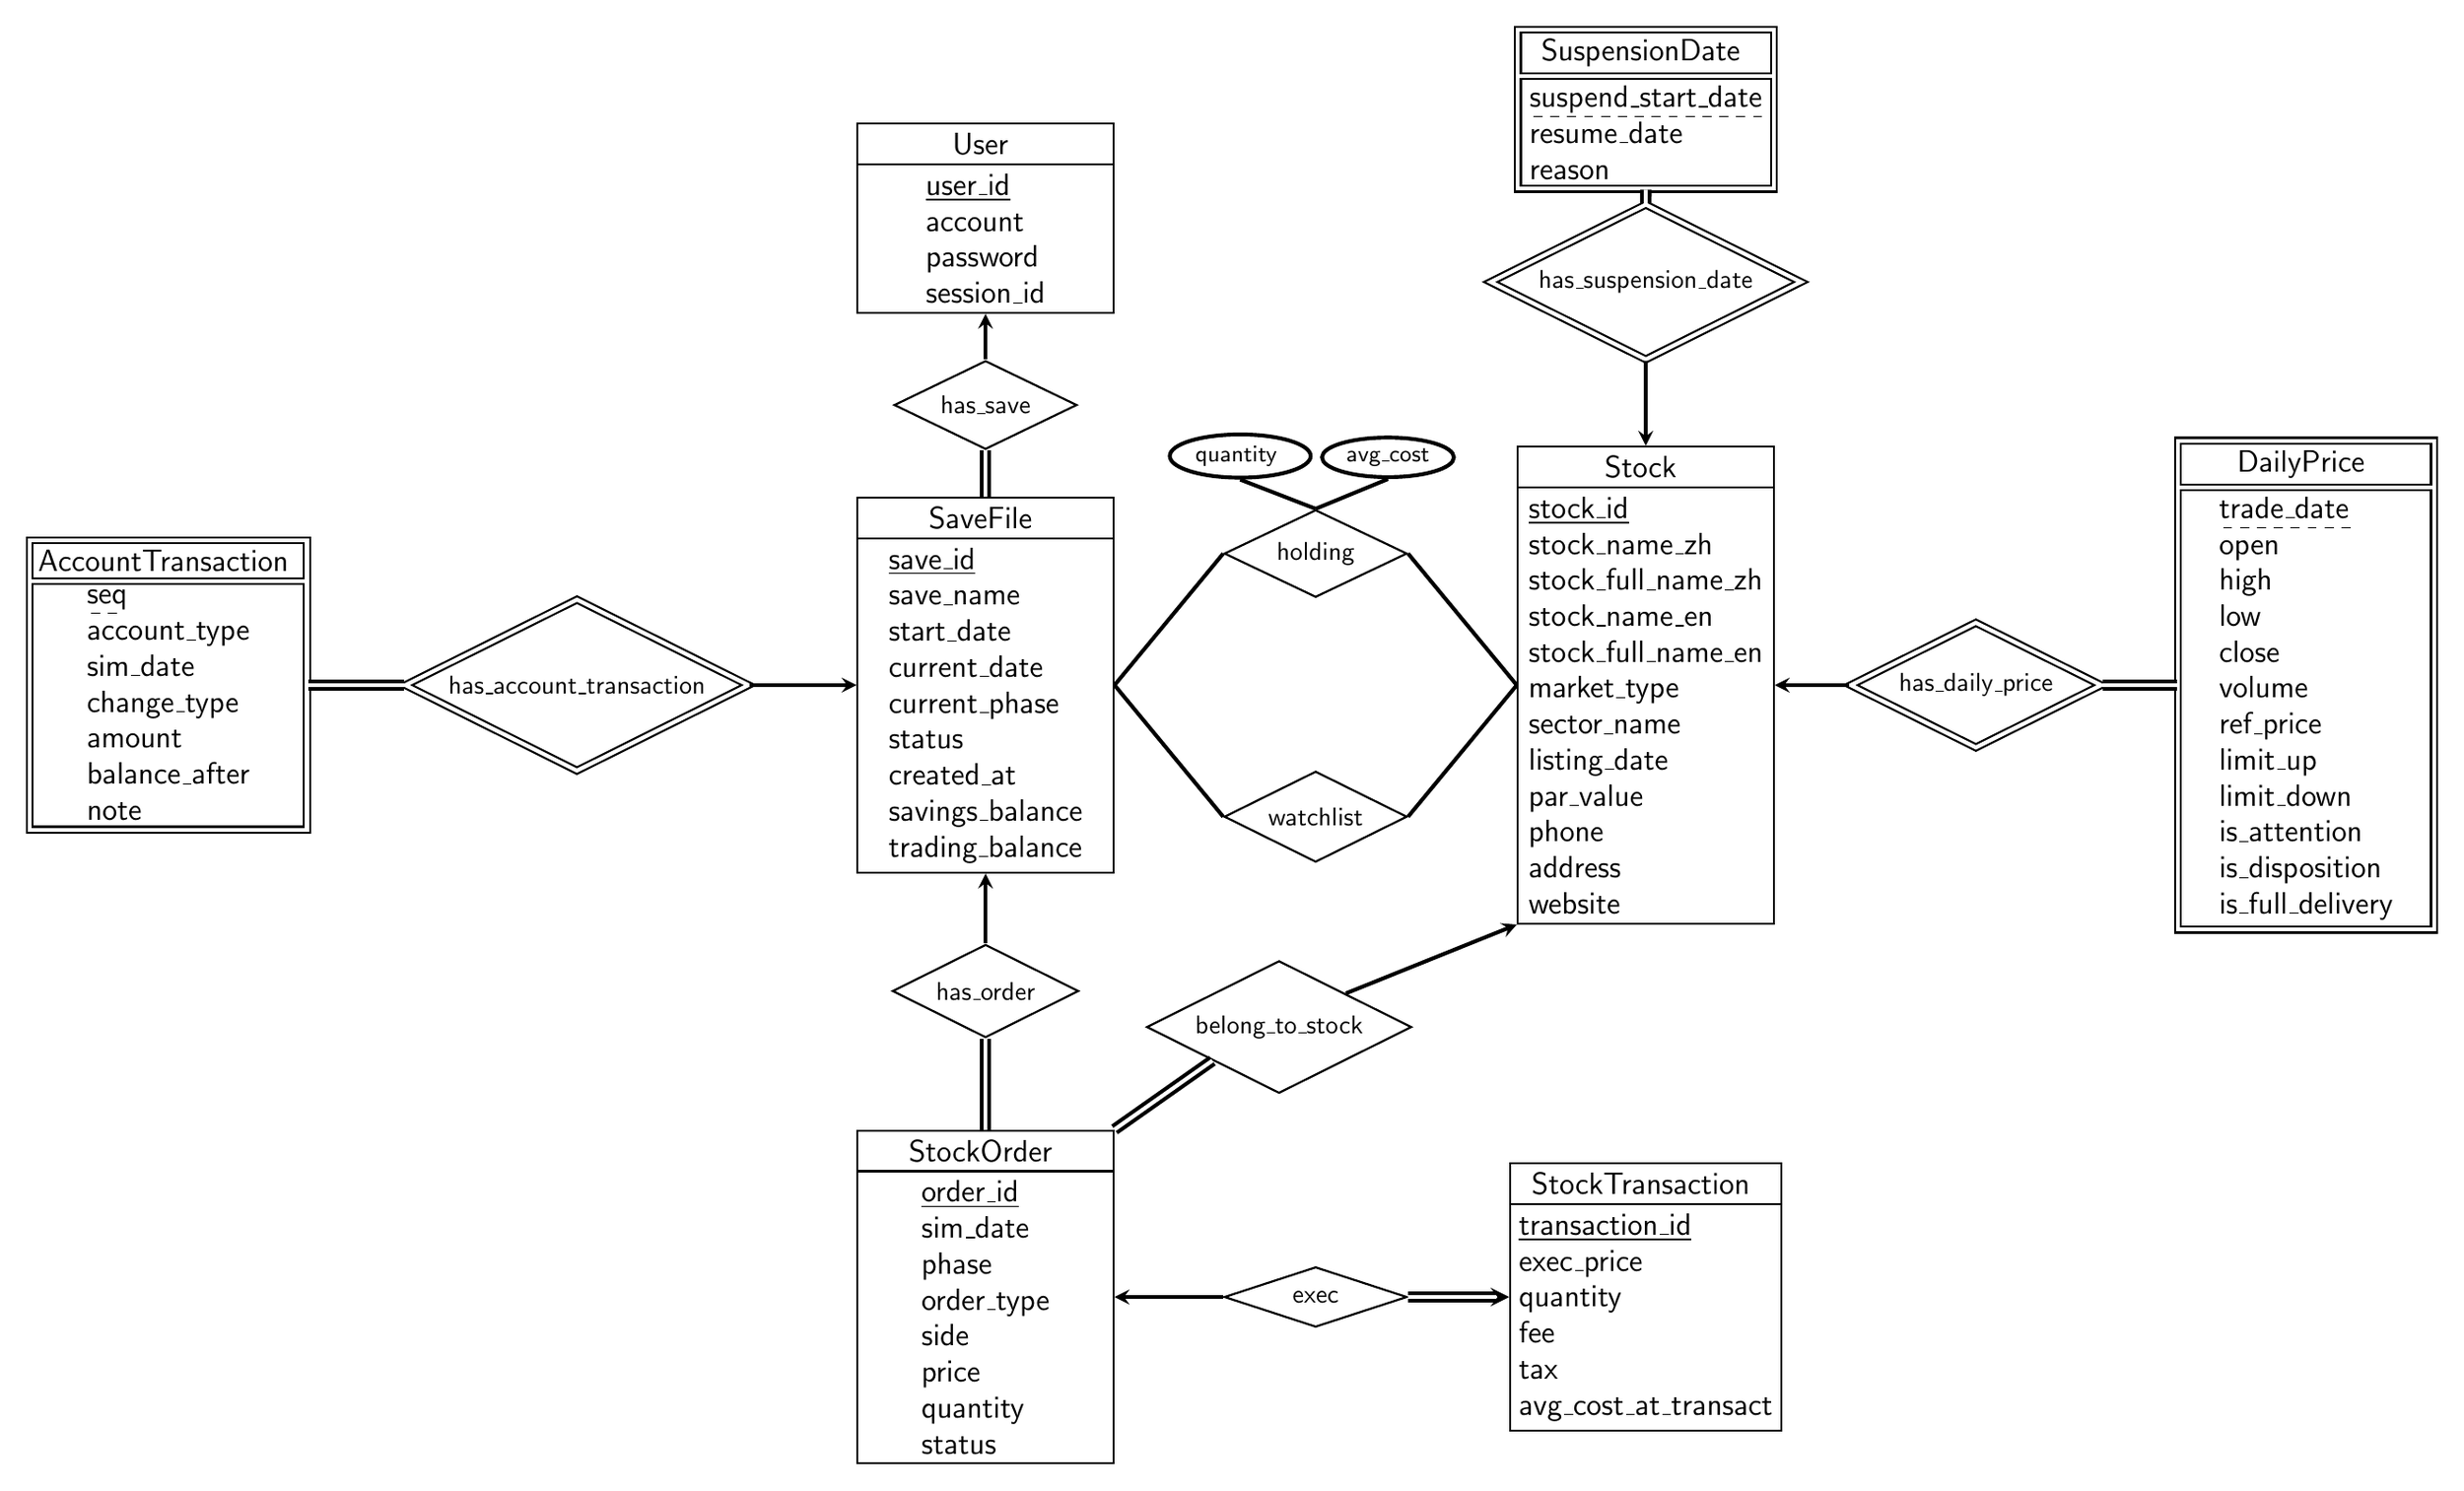
\begin{tikzpicture}[
        >=stealth,
        % 線條樣式
        every path/.style={line width=1.5pt},
        % 實體樣式 (單線方框)
        entity/.style={
            rectangle split, rectangle split parts=2,
            draw, thick, align=left, minimum width=3.5cm, font=\sffamily\large
        },
        % 弱實體樣式 (雙線方框)
        weakentity/.style={
            rectangle split, rectangle split parts=2,
            draw, thick, double, double distance=1.5pt, align=left, minimum width=3.5cm, font=\sffamily\large
        },
        % 關聯樣式 (單線菱形)
        relationship/.style={
            diamond, draw, thick, aspect=2, minimum width=2.5cm, align=center, font=\sffamily
        },
        % 弱關聯樣式 (雙線菱形)
        weakrel/.style={
            diamond, draw, thick, double, double distance=1.5pt, aspect=2, minimum width=2.5cm, align=center, font=\sffamily
        },
        % 屬性樣式
        attribute/.style={
            ellipse, draw, align=center, font=\sffamily\small, inner sep=2pt
        },
        % 連線樣式 (全參與/雙線)
        total/.style={double, double distance=1.5pt} 
    ]

        % ==========================
        % 1. 建立實體 (Entities)
        % ==========================
        
        % SaveFile (中心)
        \node[entity] (savefile) {
            \hfil SaveFile \hfil 
            \nodepart{two} 
            \underline{save\_id} \\ save\_name \\ start\_date \\ current\_date \\ 
            current\_phase \\ status \\ created\_at \\ savings\_balance \\ trading\_balance
        };

        % User (上)
        \node[entity] (user) [above=2.5cm of savefile] {
            \hfil User \hfil 
            \nodepart{two} 
            \underline{user\_id} \\ account \\ password \\ session\_id
        };

        % AccountTransaction (左) - 弱實體
        \node[weakentity] (acctrans) [left=7.5cm of savefile] {
            \hfil AccountTransaction \hfil 
            \nodepart{two} 
            \dashuline{seq} \\ account\_type \\ sim\_date \\ 
            change\_type \\ amount \\ balance\_after \\ note
        };

        % Stock (右)
        \node[entity] (stock) [right=5.5cm of savefile] {
            \hfil Stock \hfil 
            \nodepart{two} 
            \underline{stock\_id} \\ stock\_name\_zh \\ stock\_full\_name\_zh \\ stock\_name\_en \\
            stock\_full\_name\_en \\ market\_type  \\ sector\_name  \\ 
            listing\_date \\ par\_value  \\ phone  \\ 
            address \\ website 
        };

        % DailyPrice (最右) - 弱實體
        \node[weakentity] (dailyprice) [right=5.5cm of stock] {
            \hfil DailyPrice \hfil 
            \nodepart{two} 
            \dashuline{trade\_date} \\ open \\ high \\ low \\ close \\ 
            volume \\ ref\_price \\ limit\_up \\ 
            limit\_down \\ is\_attention \\ 
            is\_disposition \\ is\_full\_delivery 
        };
        
        % SuspensionDate (Stock 的上方)
        \node[weakentity] (suspension) [above=3.5cm of stock] {
            \hfil SuspensionDate \hfil 
            \nodepart{two} 
            \dashuline{suspend\_start\_date} \\ resume\_date \\ reason
        };
        % StockOrder (下)
        \node[entity] (stockorder) [below=3.5cm of savefile] {
            \hfil StockOrder \hfil 
            \nodepart{two} 
            \underline{order\_id} \\ sim\_date \\ phase \\ 
            order\_type  \\ side \\ price \\ 
            quantity  \\ status
        };

        % StockTransaction (StockOrder的右側，Stock的正下方)
        \node[entity] (stocktrans) at (stock |- stockorder) {
            \hfil StockTransaction \hfil 
            \nodepart{two} 
            \underline{transaction\_id} \\ exec\_price \\ 
            quantity  \\ fee  \\ tax \\ 
            avg\_cost\_at\_transact
        };

        % ==========================
        % 2. 建立關聯與連線
        % ==========================

        % User <-> SaveFile 
        \node[relationship] (hassave) at ($(user)!0.4!(savefile)$) {has\_save};
        \draw[<-] (user.south) -- (hassave.north);
        \draw[total] (savefile.north) -- (hassave.south);

        % SaveFile <-> AccountTransaction (弱關聯)
        \node[weakrel] (hasacctrans) at ($(savefile)!0.5!(acctrans)$) {has\_account\_transaction};
        \draw[<-] (savefile.west) -- (hasacctrans.east);
        \draw[total] (hasacctrans.west) -- (acctrans.east);

        % SaveFile <-> Stock (Holding & Watchlist)
        \path (savefile.east) -- (stock.west) coordinate[midway] (mid_ss);
        \node[relationship] (holding) at ($(mid_ss) + (0, 1.8)$) {holding};
        \node[relationship] (watchlist) at ($(mid_ss) + (0, -1.8)$) {watchlist};

        \draw (savefile.east) -- (holding.west);
        \draw (savefile.east) -- (watchlist.west);
        \draw (holding.east) -- (stock.west);
        \draw (watchlist.east) -- (stock.west);

        % Holding 屬性
        \node[attribute] (qty) [above left=0.8cm and -0.3cm of holding] {quantity };
        \node[attribute] (avgcost) [above right=0.8cm and -0.3cm of holding] {avg\_cost};
        \draw (holding.north) -- (qty.south);
        \draw (holding.north) -- (avgcost.south);

        % Stock <-> DailyPrice (弱關聯)
        \node[weakrel] (hasdailyprice) at ($(stock)!0.5!(dailyprice)$) {has\_daily\_price};
        \draw[<-] (stock.east) -- (hasdailyprice.west);
        \draw[total] (hasdailyprice.east) -- (dailyprice.west);

        % Stock <-> SuspensionDate (弱關聯)
        \node[weakrel] (hassuspension) at ($(stock)!0.7!(suspension)$) {has\_suspension\_date};
        \draw[<-] (stock.north) -- (hassuspension.south);
        \draw[total] (hassuspension.north) -- (suspension.south);

        % SaveFile <-> StockOrder
        \node[relationship] (hasorder) at ($(savefile)!0.5!(stockorder)$) {has\_order};
        \draw[<-] (savefile.south) -- (hasorder.north);
        \draw[total] (hasorder.south) -- (stockorder.north);

        % StockOrder <-> StockTransaction (exec)
        \node[relationship] (exec) at ($(stockorder)!0.5!(stocktrans)$) {exec};
        \draw[<-] (stockorder.east) -- (exec.west);
        \draw[total,->] (exec.east) -- (stocktrans.west);

        % StockOrder <-> Stock (belong_to_stock)
        % 將菱形置於兩者連線的中間偏左上角，避免線條與其他實體重疊
        \node[relationship] (belongto) at ($(stockorder.north east)!0.5!(stock.south west) + (-0.5, 0)$) {belong\_to\_stock};
        \draw[total] (stockorder.north east) -- (belongto.south west);
        \draw[<-] (stock.south west) -- (belongto.north east);

    \end{tikzpicture}
}
\end{center}
}
\section{設計概念與限制說明}
\begin{enumerate}
    \item \texttt{has\_save}: 記錄使用者擁有哪些時光機存檔。使用者（User）對時光機存檔（SaveFile）為一對多，並且時光機存檔（SaveFile）一定對應到唯一一個使用者（User）。
    \item \texttt{has\_account\_transaction}: 時光機存檔（SaveFile）對帳戶金流明細（AccountTransaction）為一對多，並且帳戶金流明細（AccountTransaction）一定對應到唯一一個時光機存檔（SaveFile）。
    \item \texttt{has\_order}: 記錄時光機存檔中擁有哪些委託單。時光機存檔（SaveFile）對委託單（StockOrder）為一對多，並且委託單（StockOrder）一定對應到唯一一個時光機存檔（SaveFile）。
    \item \texttt{exec}: 委託單（StockOrder）對股票交易紀錄（StockTransaction）為一對一，並且股票交易紀錄（StockTransaction）一定對應到唯一一個委託單（StockOrder）。
    \item \texttt{belong\_to\_stock}: 委託單（StockOrder）對股票基本面（Stock）為多對一，並且委託單（StockOrder）一定對應到唯一一個股票基本面（Stock）。
    \item \texttt{holding}: 紀錄時光機存檔中有哪些股票。時光機存檔（SaveFile）對股票基本面（Stock）為多對多。同時也記錄股票數量（quantity）和平均價。
    \item \texttt{watchlist}: 紀錄時光機存檔中關注的股票有哪些。時光機存檔（SaveFile）對股票基本面（Stock）為多對多。
    \item \texttt{has\_daily\_price} :股票基本面（Stock）對歷史日線行情（DailyPrice）為一對多，並且歷史日線行情（DailyPrice）一定對應到唯一一個股票基本面（Stock）。
    \item \texttt{has\_suspension\_date} : 股票基本面（Stock）對暫停交易日期（SuspensionDate）為一對多，並且停牌日期（SuspensionDate）一定對應到唯一一個股票基本面（Stock）。
\end{enumerate} 

\section{其他設計考量}
\begin{enumerate}
    \item 或許 SaveFile 可做為 weak entity 依賴於 User。
    
    若這樣設計：若將 SaveFile 作為 weak entity，且它又被許多 entity 依賴，會導致所有依賴於 SaveFile 的 entities 都需要 user\_id、save\_id 視為 PK。

    我們的決策：我們認為這樣操作起來較為麻煩，因此將 SaveFile 作為 strong entity。

    \item 目前委託單（StockOrder）與成交紀錄（StockTransaction）是一對一關係，但真實交易中，一筆委託單可能會分成多次成交，因此若想提高模擬真實性，可能需要改成一對多設計。
    
    本系統為簡化交易邏輯，一筆委託單只會有全部成交和全部不成交這兩種可能，因此維持一對一關係。

\end{enumerate}

\appendix
\section{附錄：Report 1}

\includepdf[
    pages={-}, 
    pagecommand={\thispagestyle{headings}}, 
    scale=0.99, 
    offset=0 -0cm % 調整 PDF 位置以避免蓋住標題
]{../report1-2/report1-2.pdf}
\end{document}